\begin{figure}[h]
\centering
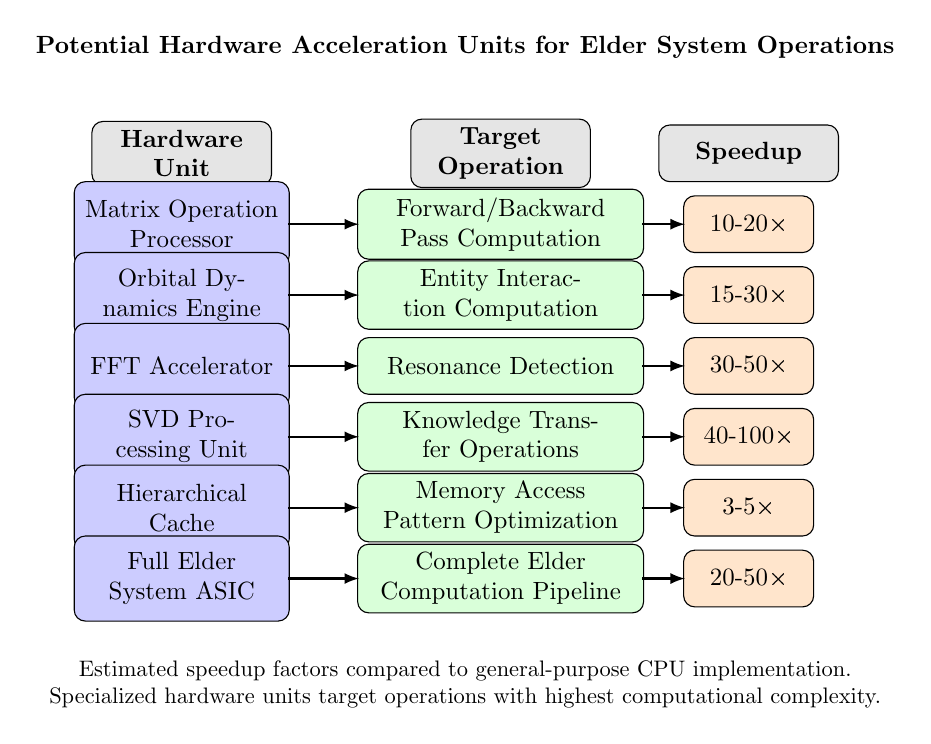
\begin{tikzpicture}[scale=0.9, transform shape]
    % Define styles
    \tikzset{
        processor/.style={draw, fill=blue!20, rounded corners, minimum width=3cm, minimum height=1.2cm, text width=2.8cm, align=center},
        operation/.style={draw, fill=green!15, rounded corners, minimum width=4cm, minimum height=0.8cm, text width=3.8cm, align=center},
        speedup/.style={draw, fill=orange!20, rounded corners, minimum width=1.8cm, minimum height=0.8cm, text width=1.6cm, align=center},
        thickarrow/.style={->, >=latex, thick},
        headerbox/.style={draw, fill=gray!20, rounded corners, minimum width=2.5cm, minimum height=0.8cm, text width=2.3cm, align=center, font=\bfseries}
    }
    
    % Headers
    \node[headerbox] at (0,6) {Hardware Unit};
    \node[headerbox] at (4.5,6) {Target Operation};
    \node[headerbox] at (8,6) {Speedup};
    
    % Row 1: Matrix Processor
    \node[processor] (mp) at (0,5) {Matrix Operation Processor};
    \node[operation] (mp_op) at (4.5,5) {Forward/Backward Pass Computation};
    \node[speedup] (mp_speed) at (8,5) {10-20×};
    
    % Row 2: Orbital Dynamics Engine
    \node[processor] (ode) at (0,4) {Orbital Dynamics Engine};
    \node[operation] (ode_op) at (4.5,4) {Entity Interaction Computation};
    \node[speedup] (ode_speed) at (8,4) {15-30×};
    
    % Row 3: FFT Accelerator
    \node[processor] (fft) at (0,3) {FFT Accelerator};
    \node[operation] (fft_op) at (4.5,3) {Resonance Detection};
    \node[speedup] (fft_speed) at (8,3) {30-50×};
    
    % Row 4: SVD Unit
    \node[processor] (svd) at (0,2) {SVD Processing Unit};
    \node[operation] (svd_op) at (4.5,2) {Knowledge Transfer Operations};
    \node[speedup] (svd_speed) at (8,2) {40-100×};
    
    % Row 5: Hierarchical Cache
    \node[processor] (cache) at (0,1) {Hierarchical Cache};
    \node[operation] (cache_op) at (4.5,1) {Memory Access Pattern Optimization};
    \node[speedup] (cache_speed) at (8,1) {3-5×};
    
    % Row 6: Elder System ASIC
    \node[processor] (asic) at (0,0) {Full Elder System ASIC};
    \node[operation] (asic_op) at (4.5,0) {Complete Elder Computation Pipeline};
    \node[speedup] (asic_speed) at (8,0) {20-50×};
    
    % Connecting lines
    \foreach \i in {5,4,3,2,1,0} {
        \draw[thickarrow] (1.5,\i) -- (2.5,\i);
        \draw[thickarrow] (6.5,\i) -- (7.1,\i);
    }
    
    % Title
    \node[align=center, font=\bfseries] at (4,7.5) {Potential Hardware Acceleration Units for Elder System Operations};
    
    % Footer explanation
    \node[align=center, scale=0.9] at (4,-1.5) {
        Estimated speedup factors compared to general-purpose CPU implementation.\\
        Specialized hardware units target operations with highest computational complexity.
    };
    
\end{tikzpicture}
\caption{Potential specialized hardware acceleration units for the Elder Heliosystem. Each hardware component targets specific operations identified through computational complexity analysis as performance bottlenecks. The estimated speedup factors represent the expected performance improvement compared to a general-purpose CPU implementation. The full Elder System ASIC would integrate all specialized units into a single coherent architecture optimized for the computational complexity profile of the Elder framework, enabling efficient scaling to larger problem dimensions.}
\label{fig:hardware_acceleration}
\end{figure}